\documentclass{standalone}
\usepackage{tikz}
\usetikzlibrary{circuits.logic.US}
\usetikzlibrary{positioning}
\usepackage{circuitikz}
\begin{document}

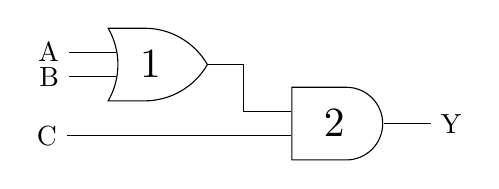
\begin{tikzpicture}[circuit logic US, scale=1.5, node distance=0.4]
	 \node [or gate, inputs=nn] (lg1) {1};
%	 \node [or gate, inputs=nn, below=of lg1 ] (lg2) {};
	 \node [and gate, inputs=nn, right=of lg1, xshift=3mm, yshift=-5mm] (lg3) {2};
	 
	 \draw (lg1.input 1) ++(left:3mm) coordinate (start);
	 \draw (lg1.input 1 -| start) -- (lg1.input 1);
	 \draw (lg1.input 2 -| start) -- (lg1.input 2);
%	 \draw (lg2.input 1 -| start) -- (lg2.input 1);
%	 \draw (lg2.input 2 -| start) -- (lg2.input 2);
	 \draw (lg1.output) -- ++(right:3mm) |- (lg3.input 1);
%	 \draw (lg2.output) -- ++(right:3mm) |- (lg3.input 2);
	 \draw (lg3.output) -- ++(right:3mm);

	 \draw (lg1.input 1) -- node[at end,left]{A} ++(left:4mm);
	 \draw (lg1.input 2) -- node[at end,left]{B} ++(left:4mm);
	 \draw (lg3.input 2) -- node[at end,left]{C} ++(left:19mm);
%	 \draw (lg2.input 2) -- node[at end,left]{D} ++(left:4mm);
	 \draw (lg3.output) -- node[at end,right]{Y} ++(right:4mm);
 \end{tikzpicture}

\end{document}